\documentclass[a4paper,12pt]{article}
\usepackage{tikz}

\begin{document}
%\begin{figure}
%  \begin{center}
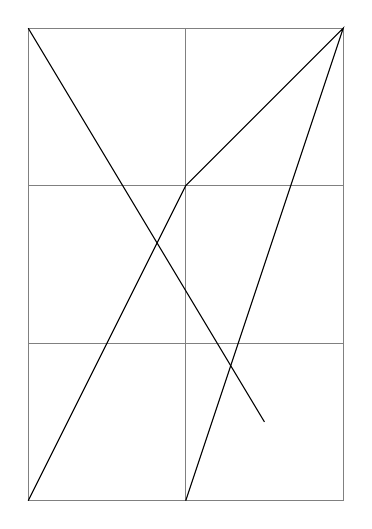
\begin{tikzpicture}[scale=2]  % scale both x and y coordinate
  \draw [help lines] (0,0) grid (2,3);
  \draw (0,0) -- (1,2) -- (2,3) -- (1,0);
  \draw (0,3) -- (1.5,0.5);
\end{tikzpicture}

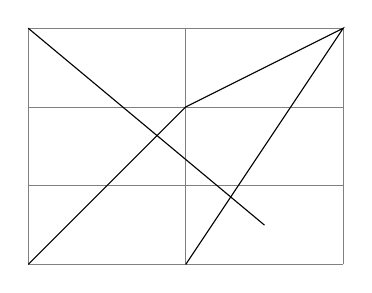
\begin{tikzpicture}[xscale=2] % scale x coordinate only
  \draw[help lines] (0,0) grid (2,3);
  \draw (0,0) -- (1,2) -- (2,3) -- (1,0);
  \draw (0,3) -- (1.5,0.5);
\end{tikzpicture}

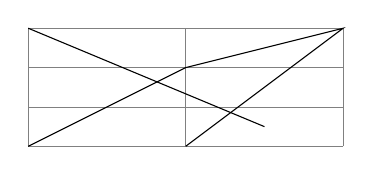
\begin{tikzpicture}[xscale=2, yscale=0.5] % scale x=2, y=0.5
  \draw[help lines] (0,0) grid (2,3);
  \draw (0,0) -- (1,2) -- (2,3) -- (1,0);
  \draw (0,3) -- (1.5,0.5);
\end{tikzpicture}

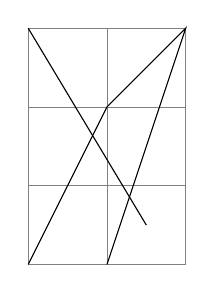
\begin{tikzpicture}
  \draw [help lines] (0,0) grid (2,3);
  \draw (0,0) -- (1,2) -- (2,3) -- (1,0);
  \draw (0,3) -- (1.5,0.5);
\end{tikzpicture}

% Arrows
\begin{tikzpicture}
  \draw [->] (0,0) -- (2,2);
  \draw [<-] (0,2) -- (2,0);
  \draw [|->] (0,1) -- (2,1);
  \draw [<->] (6,0) -- (3,0) -- (3,3);
\end{tikzpicture}

% ultra thin; very thin; thin; semithick; thick; very thick; ultra thick; help lines
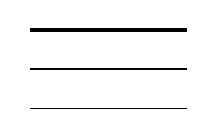
\begin{tikzpicture}
  \draw [ultra thick] (0,1) -- (2,1);
  \draw [thick] (0,0.5) -- (2,0.5);
  \draw [thin] (0,0) -- (2,0);
\end{tikzpicture}

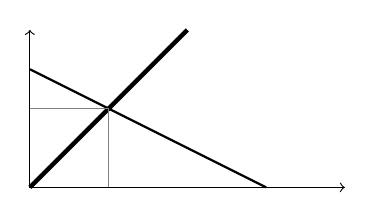
\begin{tikzpicture}
  \draw [<->] (0,2) -- (0,0) -- (4,0);
  \draw [thick] (0,1.5) -- (3,0);
  \draw [ultra thick] (0,0) -- (2,2);
  \draw [help lines] (1,0) -- (1,1) -- (0,1);
\end{tikzpicture}


\begin{tikzpicture}
  \draw [line width=12] (0,0) -- (0,2);
  \draw [line width=0.2cm] (4,0.75) -- (5,0.25);
\end{tikzpicture}

% Dashes and dots line
\begin{tikzpicture}
  \draw [dashed, ultra thick] (0,1) -- (2,1);
  \draw [dashed] (0,0.5) -- (2,0.5);
  \draw [dotted] (0,0) -- (2,0);
\end{tikzpicture}

% colors
% red, green, blue, cyan, magenta, yellow, black, gray, drakgray, lightgray, brown,
% lime, oliver, orange, pink, purple, teal, violet, white.
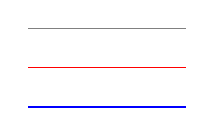
\begin{tikzpicture}
  \draw [gray] (0,1) -- (2,1);
  \draw [red] (0,0.5) -- (2,0.5);
  \draw [blue] (0,0) -- (2,0);
\end{tikzpicture}

wherever 
\begin{tikzpicture} \draw [yellow, line width=6] (0,0) -- (.5,0); \end{tikzpicture} you want

% curves
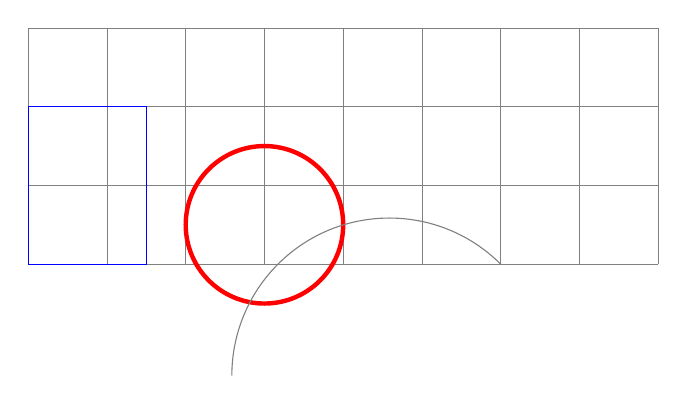
\begin{tikzpicture}
  \draw [help lines] (0,0) grid (8,3);
  \draw [blue] (0,0) rectangle (1.5,2);
  \draw [red, ultra thick] (3,0.5) circle [radius=1];
  \draw [gray] (6,0) arc [radius=2, start angle=45, end angle=180];
\end{tikzpicture}

% smoother corner
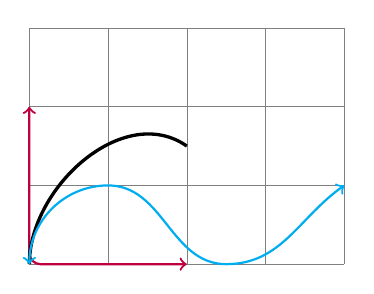
\begin{tikzpicture}
  \draw [help lines] (0,0) grid (4,3);
  \draw [<->, rounded corners, thick, purple] (0,2) -- (0,0) -- (2,0);
  % curve from (0,0) to (2,1.5) which leaves at an angle of 90 and arrive at an angle of 195
  \draw [very thick] (0,0) to [out=90, in=145] (2,1.5);
  \draw [<->, thick, cyan] (0,0) to [out=90,in=180] (1,1) to [out=0, in=180] (2.5,0) to [out=0, in=215] (4,1);
\end{tikzpicture}

% plotting function
% plot (\x, {function}).
% factorial(\x), sqrt(\x), pow(\x,y), exp(\x), ln(\x), log10(\x), log2(\x), abs(\x), mod(\x,y), round(\x), floor(\x), ceil(\x), sin(\x), sin(\x r), cos(\x), cos(\x r), tan(\x), min(\x,y), max(\x,y), rnd, e, pi;
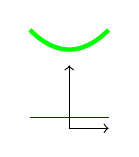
\begin{tikzpicture}
  \draw [<->] (0,0.8) -- (0,0) -- (0.5,0);
  \draw[green, ultra thick, domain=-0.5:0.5] plot (\x, {1+\x*\x});
  \draw[blue, thin, domain=-0.5:0.5] plot (\x, pi-3);
\end{tikzpicture}

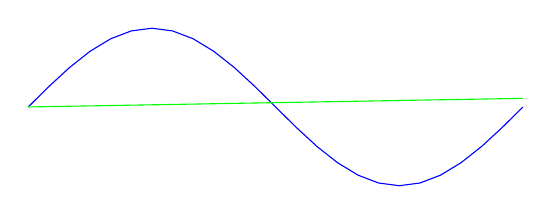
\begin{tikzpicture}
	\draw [blue, domain=0:2*pi] plot (\x, {sin(\x r)});
	\draw [green, domain=0:2*pi] plot (\x, {sin(\x)});
\end{tikzpicture}

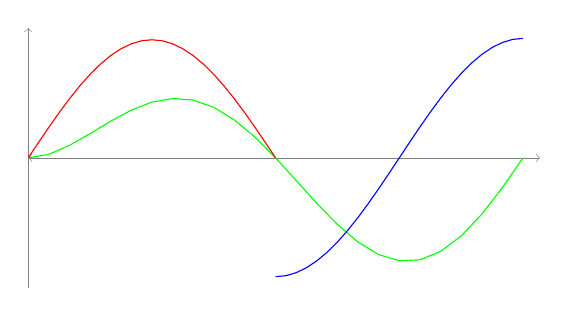
\begin{tikzpicture}[yscale=1.5]
	\draw [help lines, <->] (0,0) -- (6.5,0);
	\draw [help lines, ->] (0,-1.1) -- (0,1.1);
	\draw [green,domain=0:2*pi] plot (\x, {(sin(\x r)* ln(\x+1))/2});
	\draw [red,domain=0:pi] plot (\x, {sin(\x r)});
	\draw [blue, domain=pi:2*pi] plot (\x, {cos(\x r)*exp(\x/exp(2*pi))});
\end{tikzpicture}

% filling up space
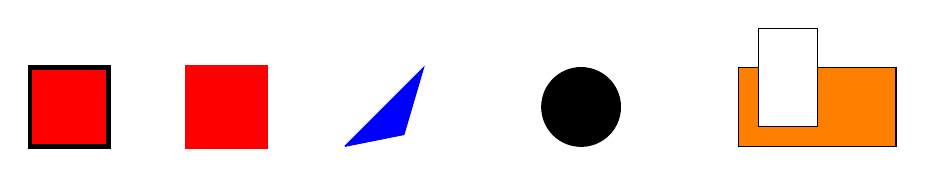
\begin{tikzpicture}
	\draw [fill=red, ultra thick] (0,0) rectangle (1,1);
  \draw [fill=red, ultra thick, red] (2,0) rectangle (3,1);
  \draw [blue, fill=blue] (4,0) -- (5,1) -- (4.75,0.15) -- (4,0);
  \draw [fill]  (7,0.5) circle [radius=0.5];
  \draw [fill=orange] (9,0) rectangle (11,1);
  \draw [fill=white] (9.25,0.25) rectangle (10,1.5);
\end{tikzpicture}


\begin{tikzpicture}
  \path [fill=gray] (0,0) rectangle (1.5,1);
  \draw [fill=gray] (2,0) rectangle (3.5,1);
\end{tikzpicture}

% mixed filling up example

\begin{tikzpicture}
  \draw [ultra thick] (0,0) to [out=90, in=150] (1,1) -- (0.85,0.15) -- (0,0);
  \draw [ultra thick, fill=purple, dotted] (2,0) to [out=90, in=150] (3,1) -- (2.85,0.15) -- (2,0);
  \path [fill=purple] (4,0) to [out=90, in=150] (5,1) -- (4.85,0.15) -- (4,0);
\end{tikzpicture}

% putting labels
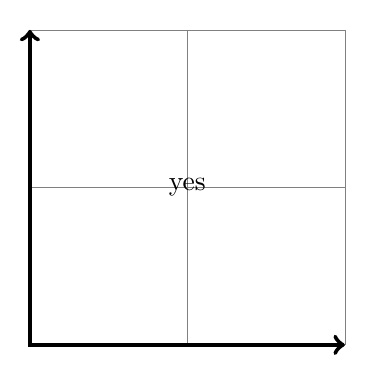
\begin{tikzpicture}[scale=2]
  \draw [help lines] (0,2) grid (2,0);
  \draw [ultra thick, <->] (0,2) -- (0,0) -- (2,0);
  \node at (1,1) {yes};
\end{tikzpicture}

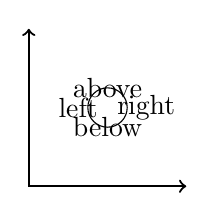
\begin{tikzpicture}
  \draw [thick, <->] (0,2) -- (0,0) -- (2,0);
  \draw (1,1) circle [radius=0.25];
  \node [below] at (1,1) {below};
  \node [above] at (1,1) {above};
  \node [right] at (1,1) {right};
  \node [left] at (1,1) {left};
\end{tikzpicture}

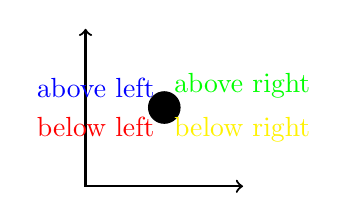
\begin{tikzpicture}
  \draw [thick, <->] (0,2) -- (0,0) -- (2,0);
  \draw [fill] (1,1) circle [radius=0.2];
  \node [below left, red] at (1,1) {below left};
  \node [below right, yellow] at (1,1) {below right};
  \node [above right, green] at (1,1) {above right};
  \node [above left, blue] at (1,1) {above left};
\end{tikzpicture}

\begin{tikzpicture}
  \draw [thick, <->] (2,0) -- (0,0) -- (0,2);
  \node [below right] at (2,0) {$x$};
  \node [above left] at (0,2) {$y$};
  \draw [fill] (1,1) circle [radius=0.05];
  \node [above right] at (1,1) {$A$};
\end{tikzpicture}

% or
\begin{tikzpicture}
  \draw [thick, <->] (2,0) node [below right] {$x$} -- (0,0) node [below left] {$O$} -- (0,2) node [above left] {$y$};
\end{tikzpicture}

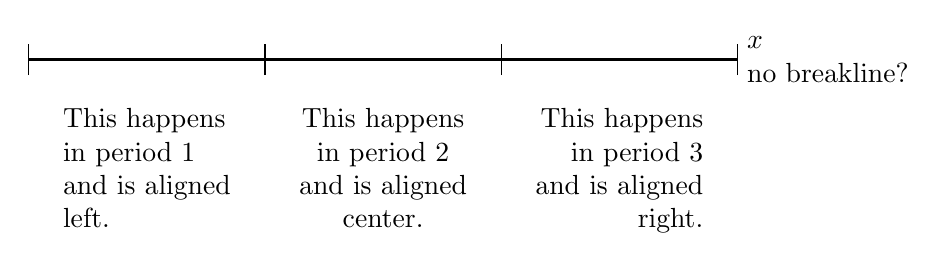
\begin{tikzpicture}
  \draw [thick] (0,0) -- (9,0);
  \draw (0,-0.2) -- (0,0.2);
  \draw (3,-0.2) -- (3,0.2);
  \draw (6,-0.2) -- (6,0.2);
  \draw (9,-0.2) -- (9,0.2);
  \node [align=left, below] at (1.5,-0.5) {This happens\\in period 1\\and is aligned\\left.};
  \node [align=center, below] at (4.5,-0.5) {This happens\\in period 2\\and is aligned\\center.};
  \node [align=right, below] at (7.5,-0.5) {This happens\\in period 3\\and is aligned\\right.};
  \node [align=left, right] at (9,0) {$x$ \\ no breakline?};
\end{tikzpicture}

%\begin{tikzpicture}
  \tikz \draw (0pt,0pt) -- (20pt,6pt);
  \tikz \fill[orange] (1,1) circle (1ex);
%\end{tikzpicture}
%wherever 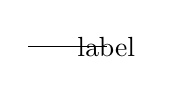
\begin{tikzpicture} \draw (0,0) -- (.5,0) node [right] {label} -- (1,0); \end{tikzpicture} you want

%    \caption{TikZ test!}
%  \end{center}
%\end{figure}

\end{document}
